% This work is licensed under the Creative Commons
% Attribution-NonCommercial-ShareAlike 4.0 International License. To view a copy
% of this license, visit http://creativecommons.org/licenses/by-nc-sa/4.0/ or
% send a letter to Creative Commons, PO Box 1866, Mountain View, CA 94042, USA.



\tikzset{every picture/.style={line width=0.75pt}} %set default line width to 0.75pt        

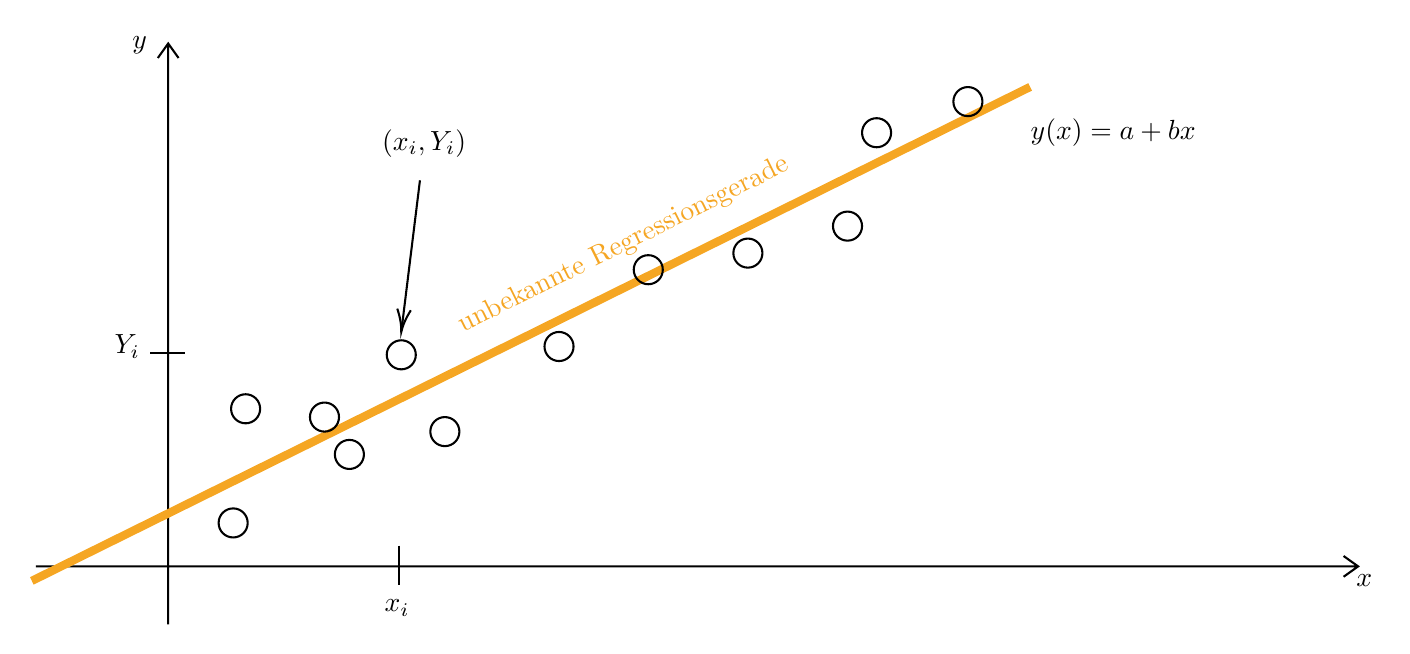
\begin{tikzpicture}[x=0.75pt,y=0.75pt,yscale=-1,xscale=1]
%uncomment if require: \path (0,300); %set diagram left start at 0, and has height of 300

%Shape: Axis 2D [id:dp07321911068108622] 
\draw  (4,261.94) -- (641,261.94)(67.7,10) -- (67.7,289.93) (634,256.94) -- (641,261.94) -- (634,266.94) (62.7,17) -- (67.7,10) -- (72.7,17)  ;
%Straight Lines [id:da07148662198339073] 
\draw [color={rgb, 255:red, 245; green, 166; blue, 35 }  ,draw opacity=1 ][line width=3]    (2,268.93) -- (483,30.93) ;


%Shape: Circle [id:dp26668633556271415] 
\draw   (92,241) .. controls (92,237.13) and (95.13,234) .. (99,234) .. controls (102.87,234) and (106,237.13) .. (106,241) .. controls (106,244.87) and (102.87,248) .. (99,248) .. controls (95.13,248) and (92,244.87) .. (92,241) -- cycle ;
%Shape: Circle [id:dp3403607469057863] 
\draw   (98,186) .. controls (98,182.13) and (101.13,179) .. (105,179) .. controls (108.87,179) and (112,182.13) .. (112,186) .. controls (112,189.87) and (108.87,193) .. (105,193) .. controls (101.13,193) and (98,189.87) .. (98,186) -- cycle ;
%Shape: Circle [id:dp4758519789604272] 
\draw   (194,197) .. controls (194,193.13) and (197.13,190) .. (201,190) .. controls (204.87,190) and (208,193.13) .. (208,197) .. controls (208,200.87) and (204.87,204) .. (201,204) .. controls (197.13,204) and (194,200.87) .. (194,197) -- cycle ;
%Shape: Circle [id:dp35126366068887793] 
\draw   (446,38) .. controls (446,34.13) and (449.13,31) .. (453,31) .. controls (456.87,31) and (460,34.13) .. (460,38) .. controls (460,41.87) and (456.87,45) .. (453,45) .. controls (449.13,45) and (446,41.87) .. (446,38) -- cycle ;
%Shape: Circle [id:dp6450412209324151] 
\draw   (402,53) .. controls (402,49.13) and (405.13,46) .. (409,46) .. controls (412.87,46) and (416,49.13) .. (416,53) .. controls (416,56.87) and (412.87,60) .. (409,60) .. controls (405.13,60) and (402,56.87) .. (402,53) -- cycle ;
%Shape: Circle [id:dp4264033728988835] 
\draw   (388,98) .. controls (388,94.13) and (391.13,91) .. (395,91) .. controls (398.87,91) and (402,94.13) .. (402,98) .. controls (402,101.87) and (398.87,105) .. (395,105) .. controls (391.13,105) and (388,101.87) .. (388,98) -- cycle ;
%Shape: Circle [id:dp41793329654483513] 
\draw   (292,119) .. controls (292,115.13) and (295.13,112) .. (299,112) .. controls (302.87,112) and (306,115.13) .. (306,119) .. controls (306,122.87) and (302.87,126) .. (299,126) .. controls (295.13,126) and (292,122.87) .. (292,119) -- cycle ;
%Shape: Circle [id:dp4914935297369122] 
\draw   (136,190) .. controls (136,186.13) and (139.13,183) .. (143,183) .. controls (146.87,183) and (150,186.13) .. (150,190) .. controls (150,193.87) and (146.87,197) .. (143,197) .. controls (139.13,197) and (136,193.87) .. (136,190) -- cycle ;
%Shape: Circle [id:dp23764538796154067] 
\draw   (173,160) .. controls (173,156.13) and (176.13,153) .. (180,153) .. controls (183.87,153) and (187,156.13) .. (187,160) .. controls (187,163.87) and (183.87,167) .. (180,167) .. controls (176.13,167) and (173,163.87) .. (173,160) -- cycle ;
%Shape: Circle [id:dp6151497769773182] 
\draw   (249,156) .. controls (249,152.13) and (252.13,149) .. (256,149) .. controls (259.87,149) and (263,152.13) .. (263,156) .. controls (263,159.87) and (259.87,163) .. (256,163) .. controls (252.13,163) and (249,159.87) .. (249,156) -- cycle ;
%Shape: Circle [id:dp6112008925466065] 
\draw   (148,208) .. controls (148,204.13) and (151.13,201) .. (155,201) .. controls (158.87,201) and (162,204.13) .. (162,208) .. controls (162,211.87) and (158.87,215) .. (155,215) .. controls (151.13,215) and (148,211.87) .. (148,208) -- cycle ;
%Shape: Circle [id:dp7443465654150703] 
\draw   (340,111) .. controls (340,107.13) and (343.13,104) .. (347,104) .. controls (350.87,104) and (354,107.13) .. (354,111) .. controls (354,114.87) and (350.87,118) .. (347,118) .. controls (343.13,118) and (340,114.87) .. (340,111) -- cycle ;
%Straight Lines [id:da5984247302071123] 
\draw    (179,251.93) -- (179,270.93) ;


%Straight Lines [id:da6676175412533971] 
\draw    (59,158.93) -- (76,158.93) ;


%Straight Lines [id:da2593592347170056] 
\draw    (189,75.93) -- (180.24,147.02) ;
\draw [shift={(180,149)}, rotate = 277.02] [color={rgb, 255:red, 0; green, 0; blue, 0 }  ][line width=0.75]    (10.93,-3.29) .. controls (6.95,-1.4) and (3.31,-0.3) .. (0,0) .. controls (3.31,0.3) and (6.95,1.4) .. (10.93,3.29)   ;


% Text Node
\draw (523,53) node   {$y( x) =a+bx$};
% Text Node
\draw (287,107) node [rotate=-333.51] [align=left] {\textcolor[rgb]{0.96,0.65,0.14}{unbekannte Regressionsgerade}};
% Text Node
\draw (644,269) node   {$x$};
% Text Node
\draw (54,11) node   {$y$};
% Text Node
\draw (178,282) node   {$x_{i}$};
% Text Node
\draw (48,156) node   {$Y_{i}$};
% Text Node
\draw (191,58) node   {$( x_{i} ,Y_{i})$};


\end{tikzpicture}



